\documentclass[12pt]{article}
\usepackage[margin=1in]{geometry} %1 inch margins
\usepackage{verbatim} %multi-line comment
\usepackage{graphicx} %graphics
\usepackage{fancyhdr} %custom header
\usepackage{amsmath} %math
\usepackage{amssymb} %math symbols
\usepackage{bm} %bold math text
\usepackage{bbm} %indicators
\usepackage{soul} %for underlining
\usepackage{listings}
\usepackage{booktabs}
%\pagenumbering{gobble} %no page numberings
\pagestyle{fancy}
\newcommand{\indep}{\raisebox{0.05em}{\rotatebox[origin=c]{90}{$\models$}}}
\allowdisplaybreaks

\renewcommand{\headrulewidth}{0pt}
\lhead{CS 208 - Applied Privacy for Data Science\\Harvard University}
\rhead{Huang, Jason\\Homework 2}
%%%%%%%%%%% BEGIN DOCUMENT
\begin{document}
\begin{center}
	{\Large \textbf{CS 208 - Applied Privacy for Data Science}}\\
	{\Large \textbf{Homework 2}}\\
	\vspace*{0.1in}
	Jason Huang\\
	Spring 2019 - Harvard University\\
\end{center}

The public Github repo containing all work is at https://github.com/TurboFreeze/cs208hw. All code has also been included in the appendix of this PDF as specified.\\

{\large\textbf{Problem 1}}

\textbf{(a)}
\begin{enumerate}
	\item[(i)] The clamping function is effectively applying a post-processing function to the noisy query result. In other words, Laplace noise is added to the true mean $\bar{x}$, which must be $(\epsilon, 0)$-DP. The following clamping function does not change the privacy characteristics guaranteed by differential privacy, meaning that this mechanism \textbf{meets the definition} of $(\epsilon, 0)$-DP (following directly by privacy under post-processing and the proof of Laplace DP).
	
	Note that the scale factor parameter of the Laplace distribution should be set to $s = GS_q/\epsilon$ for differential privacy, meaning that $\epsilon = GS_q/s$. In this case, the global sensitivity $GS_q$ is the maximum change that can be affected to the statistic by a single entry's change, which in this case would be $1/n$ for the mean. Furthermore $s = 2 / n$. The $\epsilon = (1/n) / (2/n) \implies \boxed{\epsilon= 0.5}$.
	\item[(ii)] Constant ratios of Laplace mechanisms
	\item[(iii)] 
	\begin{align*}
		\dfrac{P[M(x', q) = r]}{P[M(x, q)=r]} &= \\
	\end{align*}
	\item[(iv)] 
\end{enumerate}
\begin{align*}
	P[M(x, q) = r] &= P[[\bar{x} + Z]^1_0 = r]\\
	&= \\
	\dfrac{P[M(x, q) = r]}{P[M(x', q)=r]} &= \\
	P[M(x, q) = r] &= P[\bar{x} + [Z]^1_{-1} = r]\\
	&= \\
\end{align*}

{\large\textbf{Problem 2}}

\textbf{(a)} The DGP is the following likelihood of some data vector $k\in\mathbb{N}^n$:
\[P(\mathbf{x} = \mathbf{k}) = \prod\limits^n_{i=1} \dfrac{10^{\mathbf{k}_i}e^{-10}}{\mathbf{k}_i!}\]
The DGP function was implemented using a Poisson random draw.

\emph{See the attached R script \texttt{q2.R} for the implementation}.\\

\textbf{(b)} The first mechanism was chosen, involving clamping after Laplace noise has been added.

\emph{See the attached R script \texttt{q2.R} for the implementation}.\\

\textbf{(c)} The optimal value $b^*$ for $b$ is $\boxed{b^* \approx 10}$. As expected, root mean squared error is indeed high with small clamping regions and decreases as it becomes more appropriate, with large clamping regions yielding high RMSE again.

\begin{center}
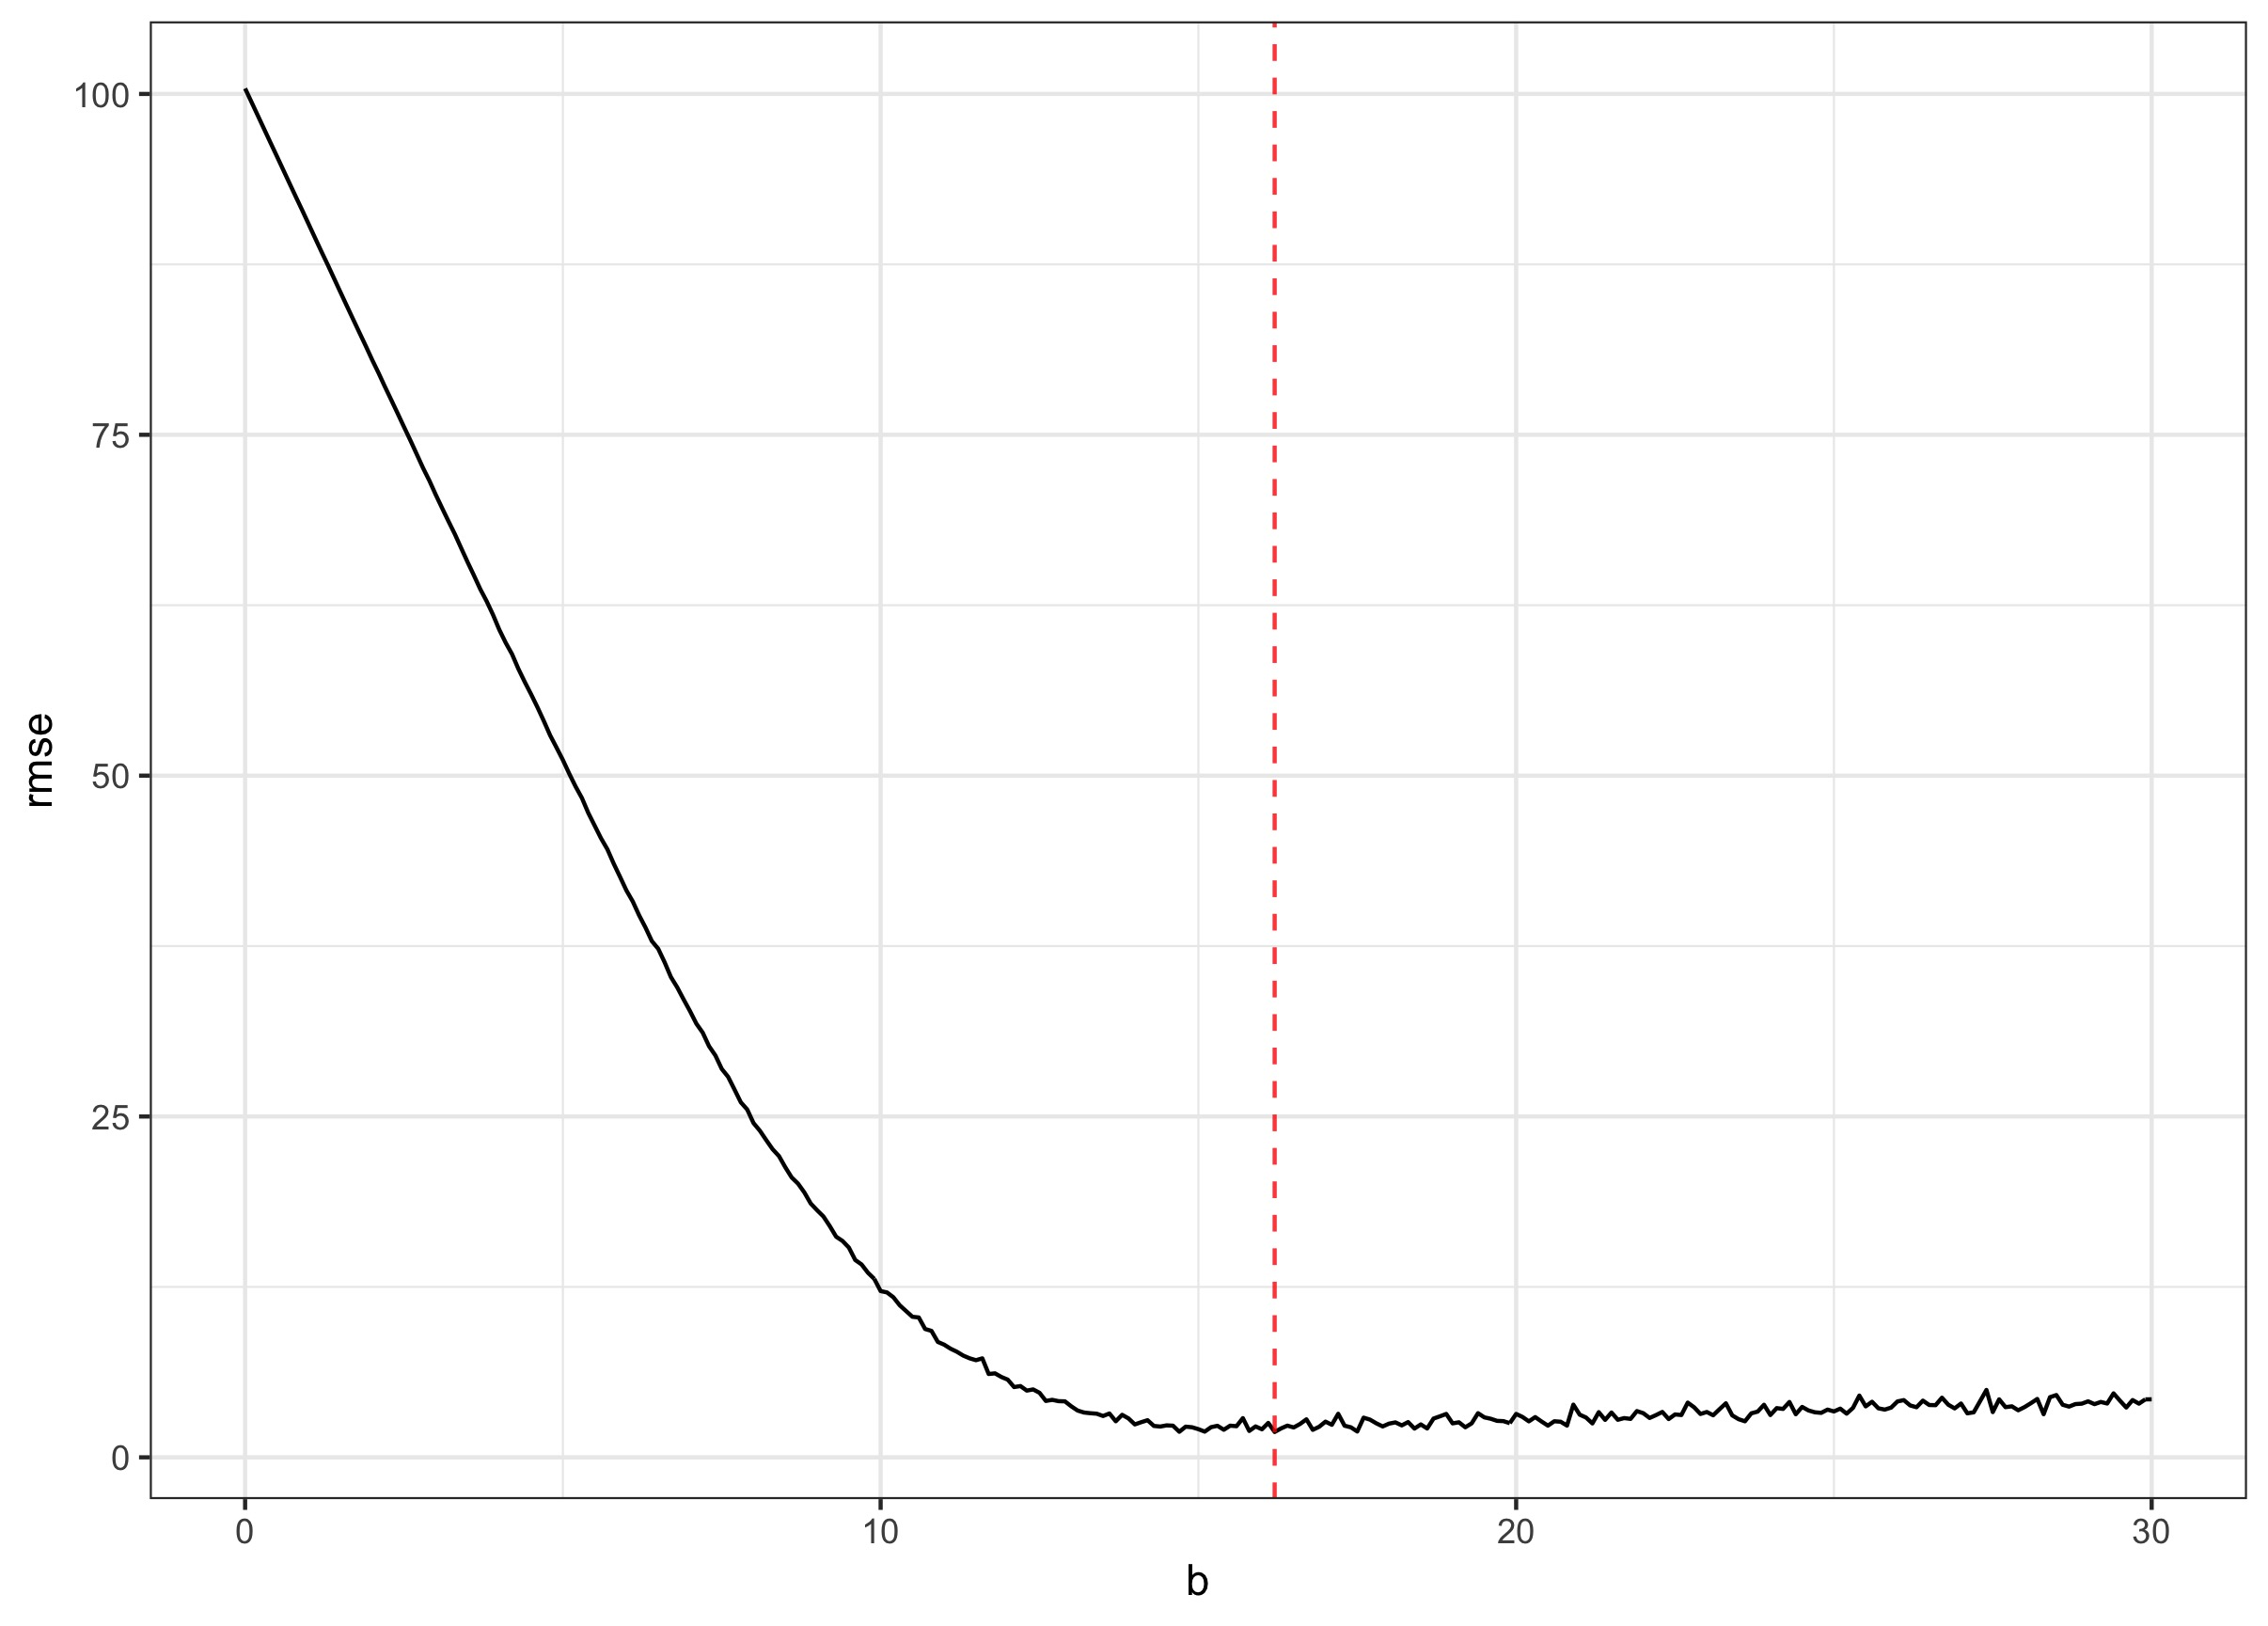
\includegraphics[width=0.7\textwidth]{clamping}
\end{center}

\emph{See the attached R script \texttt{q2.R} for the implementation}.\\

\textbf{(d)}

\textbf{(e)}\\

{\large\textbf{Problem 3}}

\textbf{(a)} There are differentially private techniques to release the means $\bar{y}$ and $\bar{x}$ as well as the slope $\hat{\beta}$. However, given the careful considerations needed for the slope $\hat{\beta}$, it may be challenging to come up with a single differentially private mechanism to derive the intercept estimate. However $\hat{\alpha} = \bar{y} - \hat{\beta}\bar{x}$ lends itself nicely to privacy preservation under composition and post-processing. Since there are three differentially private statistics needed here of $\bar{x}, \bar{y}, \hat{\beta}$, for a total epsilon budget of $\epsilon_t$, then calculate differentially private releases of each statistic with $\epsilon = \epsilon_t/3$ to yield $(\epsilon_t / 3,0)$-DP statistics. Since post-processing is allowed without affecting privacy, then this three differentially private statistics will lead to $\epsilon_t / 3 + \epsilon_t / 3 + \epsilon_t / 3 = \epsilon_t$ differential privacy for $\hat{\alpha}$ by composition and $\epsilon_t/3$ differential privacy for $\hat{\beta}$ (which is used in $\hat{\alpha}$ and does not require separate consumption of the budget). Therefore, the overall method for computing both $\hat{\alpha}$ and $\hat{\beta}$ would be $\epsilon_t$-DP, as desired.

Since the data $x_i$ is generated by a Poisson process according to the previous problem, it can be clamped using the optimal value of $b^*\approx 10$ found before. Since there is a linear relationship between $x_i$ and $y_i$ here (and it is known in the following part that the slope is simply 1), then similarly clamp $y_i$ by $b^* \approx 10$.

\emph{See the attached R script \texttt{q3.R} for the implementation}.\\

\textbf{(b)} 

\emph{See the attached R script \texttt{q3.R} for the implementation}.\\

\textbf{(c)} 

\emph{See the attached R script \texttt{q3.R} for the implementation}.\\

{\large\textbf{Problem 4}}

Use linearity of expectations and fundamental bridge to convert between probabilities and expectation of indicators.
\begin{align*}
	\mathbb{E}[\#\{ i\in [n]: A(M(X))_i = X_i\} / n] &= \mathbb{E}[\mathbbm{1}\{ i\in [n]: A(M(X))_i = X_i\} / n]\\
	&= \mathbb{E}[\sum\limits^n_{i=1}\mathbbm{1}(A(M(X))_i = X_i) / n]\\
	&= \dfrac{1}{n}\sum\limits^n_{i=1}\mathbb{E}[\mathbbm{1}(A(M(X))_i = X_i)]\\
	&= \dfrac{1}{n}\sum\limits^n_{i=1}P(A(M(X))_i = X_i)
\end{align*}
Use the definition of $(\epsilon, \delta)$-DP



\pagebreak

{\large\textbf{Appendix}}

\textbf{Code for Problem 1}

\begin{lstlisting}[language=R]
\end{lstlisting}

\pagebreak

\textbf{Code for Problem 2}

\begin{lstlisting}[language=R]
\end{lstlisting}


\pagebreak

\textbf{Code for Problem 3}

\begin{lstlisting}[language=R]
\end{lstlisting}


\end{document}